\documentclass{article}
\usepackage{amsmath}
\usepackage{amssymb}
\usepackage{amsthm}
\usepackage{thmtools}
\usepackage{cases}
\usepackage{enumitem}
\usepackage{xcolor}
\usepackage{cancel}
\usepackage{cite}
\usepackage{graphicx}
\usepackage{float}

\usepackage{algorithm2e}
\RestyleAlgo{ruled}
\SetKwComment{Comment}{/* }{ */}

\usepackage{geometry}
\geometry{margin=4cm, vmargin=3cm}

\setlength\parindent{0pt}

\title{Asian options pricing}
\author{David Castro \qquad Maxime Leroy}
\date{15 Januray 2024}

\begin{document}
\maketitle

\section*{Introduction}

An Asian option is any option with payoff of the form:
\[
	\left( S_t \right)_{t \in [0, T]} \mapsto g \left( S_T, A_T \right) \quad \text{with} \quad A_T := \frac{1}{T} \int_0^T S_u du
\]
where $\left( S_t \right)_t$ denotes the trajectory of the underlying and $T$ is the maturity of the option.
For instance, a \textit{fixed-strike} Asian call has $g(x, a) := e^{-rT} \left[ a - K \right]_+$ where $K$ denotes the strike
and a \textit{floatting-strike} Asian call has $g(s, a) := e^{-rT}  \left[ s - a \right]_+$.
In the first case, the option is exercised by its owner
if the underlying has lied above the strike \textbf{on average} throughout its lifetime. In the second case,
it is worth exercising it when the underlying is above its average value at expiry.

\

This work studies different pricing techniques for Asian options and will tackle \textbf{only fixed-strike Asian calls}
for simplicity. Furthermore, we will use Black-Scholes model. In that context, simulating $S_T$ is straightforward
and the real challenge consists in simulating $A_T$. That is why our developments for fixed-strike Asian calls
adapt directly to any Asian option of the form given above.

\

We first introduce and implement different Monte-Carlo approaches as developed by Lambert et al. \cite{main}
and B. Bouchard \cite{Bouchard}. We then compare them with a PDE approach as presented by
Rogers et al. \cite{Rogers}.

\section{Naive approach}

The most basic Monte-Carlo approach to the problem consists in approximating the integral
of the underlying over its trajectory by a Riemann sum.

\[
	A_T \approx \bar A_T^{r, m} := \frac{h}{T} \sum_{k=0}^{m-1} \bar S_{t_k}^m
	= \frac{1}{m} \sum_{k=0}^{m-1} \bar S_{t_k}^m \quad \text{with} \quad h = \frac{T}{m}
\]

where $\bar S_{t_k}^m$ denotes the $k$-th step of an Euler scheme. That gives the following estimate:

\begin{equation}
	C_r := e^{-rT} \sum_{i=1}^n \left[ \frac{1}{m} \sum_{k=0}^{m-1} \bar S_{t_k}^{m, i} - K \right]_+
	\tag{1}
\end{equation}

where $\left( \bar S^{m, i} \right)_{i = 1, \dots, n}$ are independent and identically distributed copies of $\bar S^m$.
%According to B. Bouchard \cite{Bouchard}, scheme (1) has a weak error in $O \left( \frac{1}{n} \right)$.

\

The variance is in $O \left( \dots \right)$ and the biais is in $O \left( \dots \right)$. Figure 1 shows the result
of this method for different values of $K$, $T$ and $\sigma$ where we took $n =10,000$ and $m=100$.
One can already notice that it tallies with the common idea that Asian call are cheaper than European call
for a given set of parameters. Also, quite intuitively, the gap widens when $\sigma$ and $T$ grow: the smaller
both of them are, the closer to the initial value the underlying will remain, leading to $A_T \approx S_T \approx S_0$
on average.

\begin{figure}[H]
  %\centering
  \hspace*{-0.02\linewidth}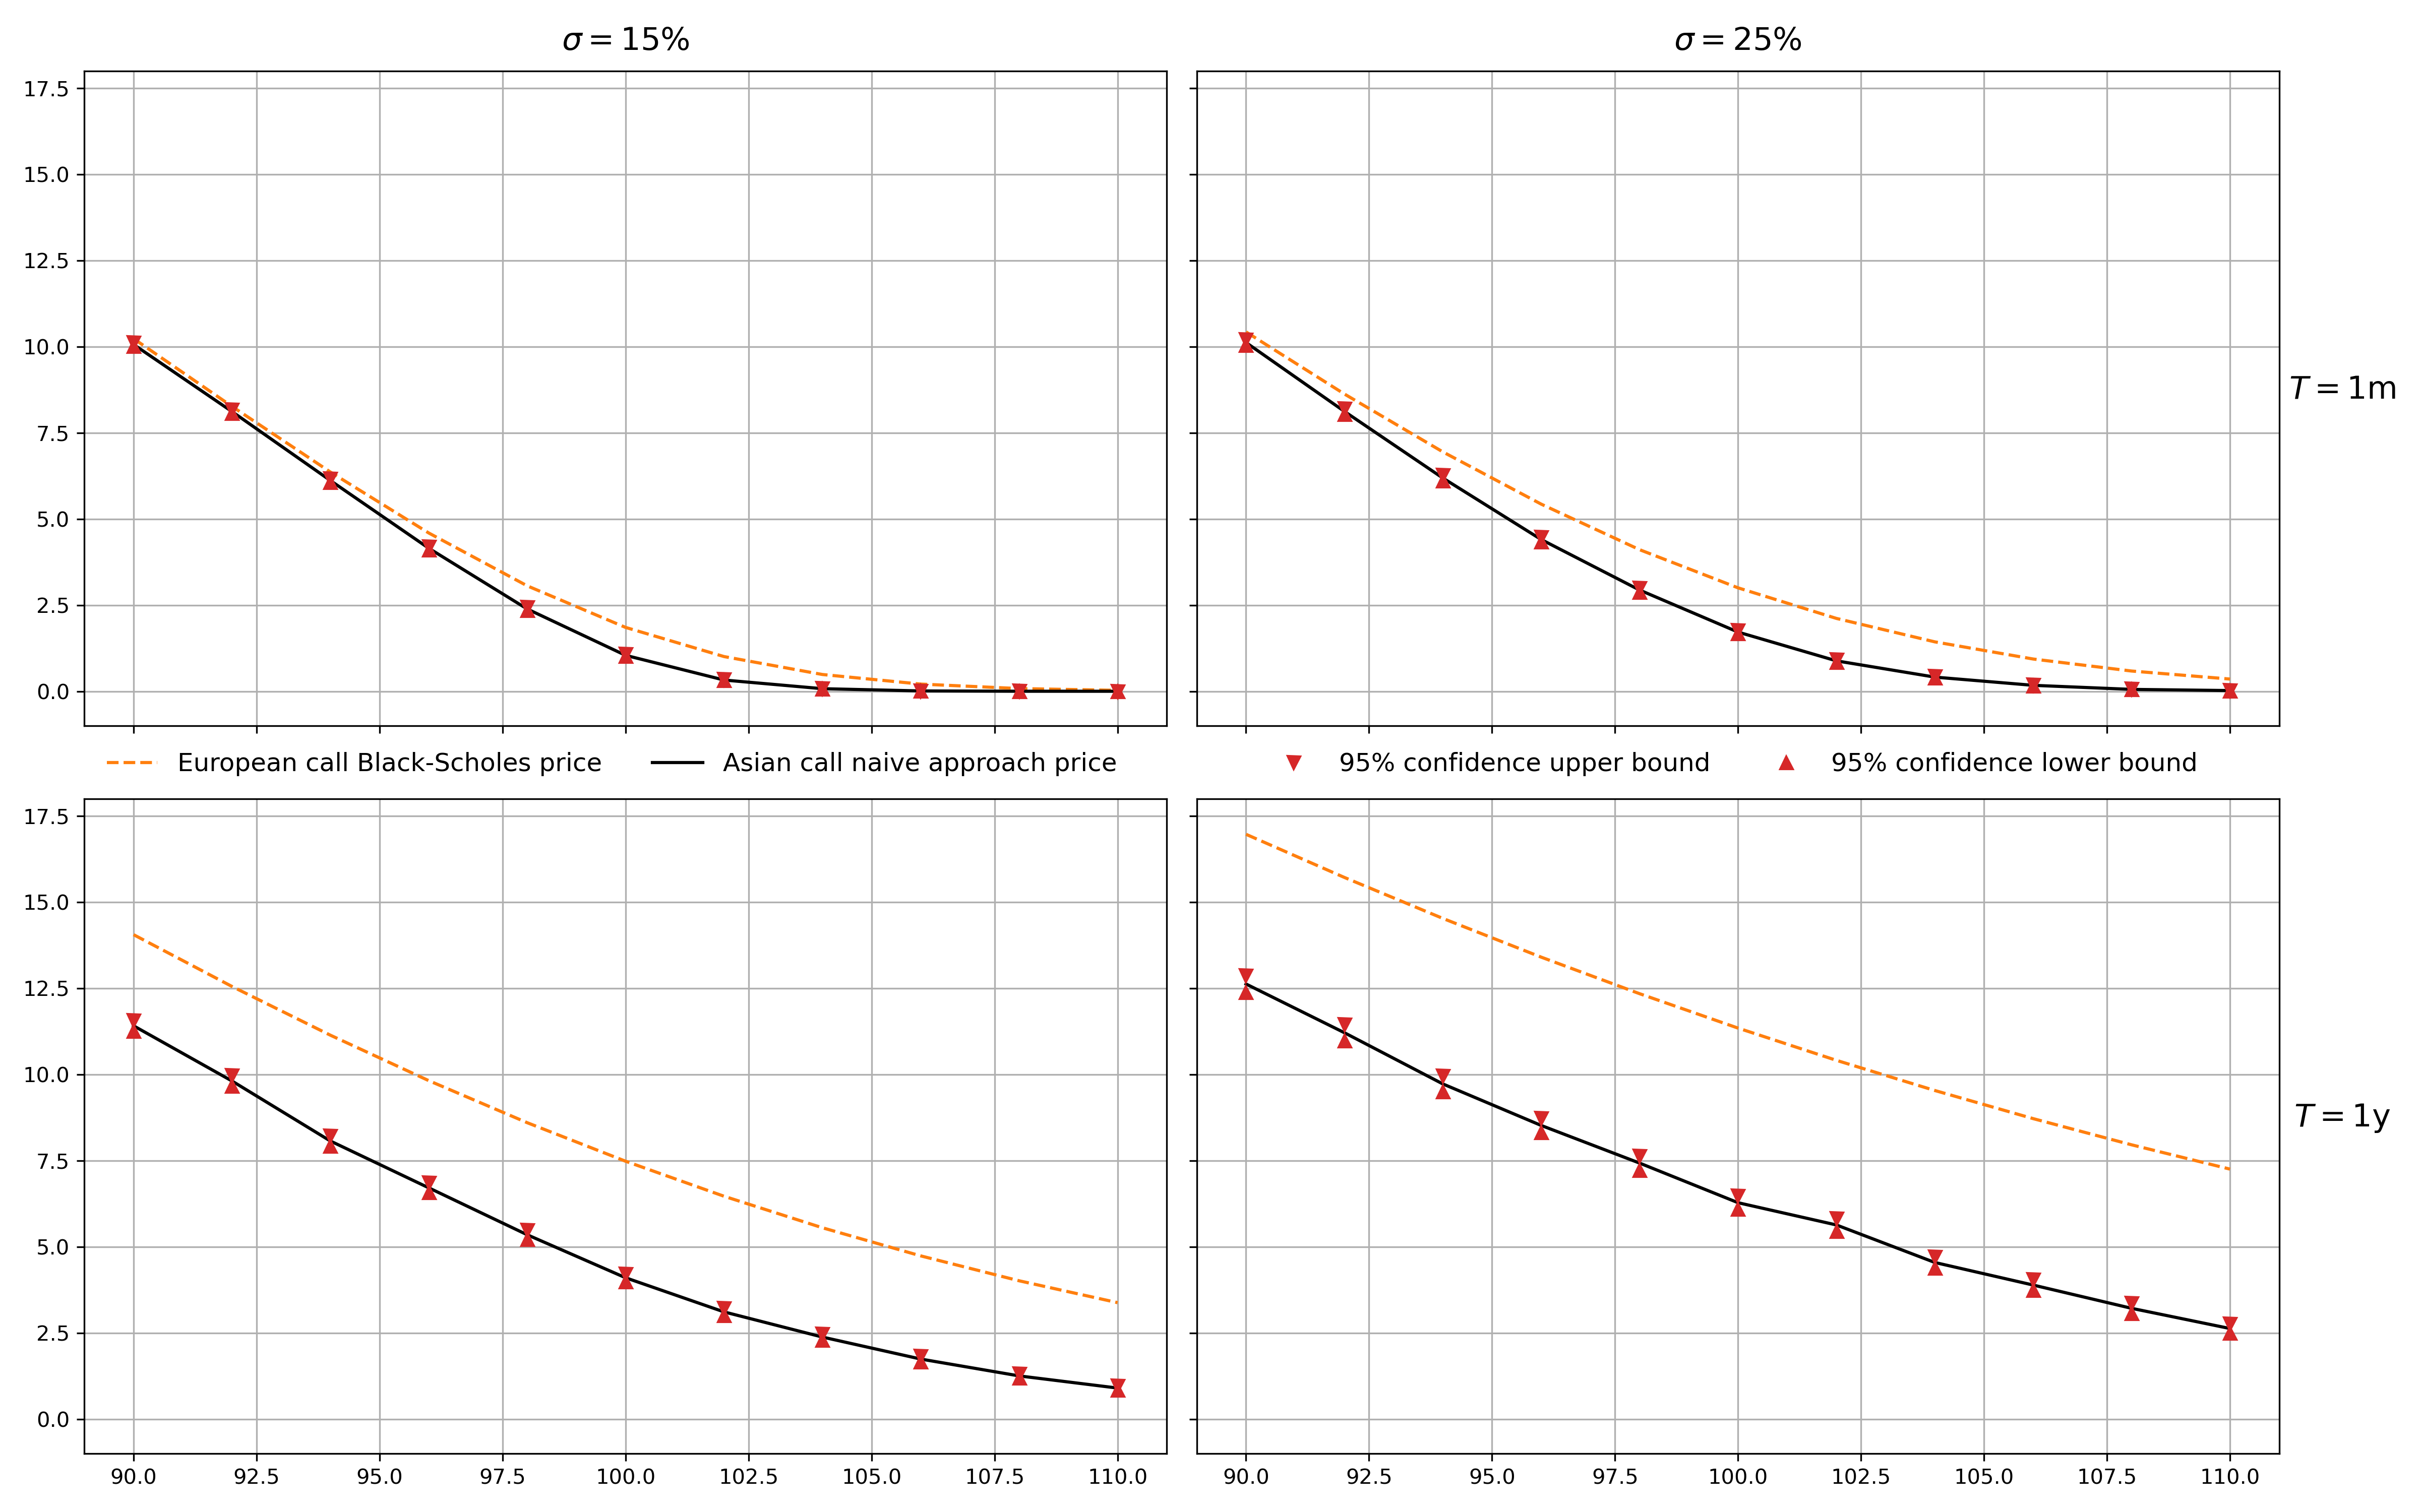
\includegraphics[width=1.065\textwidth]{charts/prices.png}
  \caption{Fixed-strike Asian call naive pricing for different values of $K$, $\sigma$ and $T$}
\end{figure}

However, these charts, particularly the one for $\sigma = 25\%$ and $T=1$y, reveal some fluctuations with
a greater magnitude than the length of the $95\%$ confidence intervals plotted in red. This stems from the bias
introduced by the approximation of $A_T$, that the figure does not reflect. This seems to be the main flaw of the
naive approach: even if the variance already looks satisfactory, the bias increases rapidly with the parameters, which
yields imprecise results.

\

The following models all give similar charts. In the below, we rather focus on the graphical representation
of the convergence properties of each scheme. As suggested in the previous paragraph, this is
the main challenge that the following approaches mean to address.

\section{Improved Monte-Carlo approaches}
\subsection{Two finer approximations}

A first improvement of the above approach proposes to better use the information provided by the simulation
$\bar S_0^m, \bar S_{t_1}^m, \dots, \bar S_T^m$ to approximate the integral $A_T$.
It relies on the fact that once the trajectory has been simulated, the best estimation of the price is:
\[
	\bar C^m := \mathbb E \left[ e^{-rT} \left[ A_T - K \right]_+ \mid \bar S_0^m, \bar S_{t_1}^m, \dots, \bar S_T^m \right]
\]

By the tower property, the expectation (estimated by a Monte-Carlo method with $n$ trajectories)
of this conditional expectation is the price of the Asian call.
At this stage, this quantity is not known either. \cite{main} introduces the following simplification:

\begin{equation}
	\bar C^m \approx e^{-rT}  \left[ \mathbb E \left[A_T
		\mid \bar S_0^m, \bar S_{t_1}^m, \dots, \bar S_T^m \right] - K \right]_+
	\tag{S}
\end{equation}

A first-order Taylor expansion leads to the additional approximation below:
\begin{align*}
	\mathbb E \left[ \int_{t_k}^{t_{k+1}} S_u du \mid \bar S_0^m, \bar S_{t_1}^m, \dots, \bar S_T^m \right]
	&= \int_{t_k}^{t_{k+1}} \mathbb E \left[ S_u \mid \bar S_{t_k}^m, \bar S_{t_{k+1}}^m \right] du \\
	&= \bar S_{t_k}^m \int_{t_k}^{t_{k+1}} \mathbb E \left[ \frac{S_u}{\bar S_{t_k}^m}
		\ \Big\vert \ \bar S_{t_k}^m, \bar S_{t_{k+1}}^m \right] du \\
	&\approx
		\bar S_{t_k}^m \int_{t_k}^{t_{k+1}} \left\{ 1 + \ln \mathbb E \left[ \frac{S_u}{\bar S_{t_k}^m}
		\ \Big\vert \ \bar S_{t_k}^m, \bar S_{t_{k+1}}^m \right] \right\} du
\end{align*}
for all $k \in \{ 0, \dots, m - 1 \}$. On the one hand, Black-Scholes model gives:
\[
	S_u \mid \bar S_{t_k}^m, \bar S_{t_{k+1}}^m = \bar S_{t_k}^m \exp
	\left\{ \left( r - \frac{\sigma^2}{2} \right) (u - t_k) + \sigma
	\left ( \left( W_u \mid \bar W_{t_k}^m, \bar W_{t_{k+1}}^m \right) - \bar W_{t_k}^m \right) \right\}
\]
where $\bar W_{t_k}^m$ is the $k$-th step of the Brownian Motion used to simulate $\bar S^m$ as
part of the Euler scheme, ie:
$\bar S_{t_k}^m = S_0 \exp \{ ( r - \frac{\sigma^2}{2} ) t_k + \sigma \bar W_{t_k}^m \}$.
On the other hand, $W_u \mid \bar W_{t_k}^m, \bar W_{t_{k+1}}^m$ follows a Brownian Bridge.
Therefore, the integrand has an analytical expression indeed and it yields the following scheme:

\begin{equation}
    A_T \approx \bar A_T^{e, m} = \frac{1}{m} \sum_{k=0}^{m-1} \bar S_{t_k}^m
    	\left( 1 + \frac{rh}{2} + \sigma \frac{\bar W_{t_{k+1}}^m - \bar W_{t_k}^m}{2} \right) \tag{2}
\end{equation}

The above development is actually equivalent to a trapezoidal method in comparison with the more
basic Riemann sum used in scheme $(1)$. We note $C_e$ the corresponding estimate of the price.

\

Instead of simplification (S), \cite{Bouchard} and \cite{main} suggest a quite similar approach. For each step
of the Monte-Carlo estimation, first fix a trajectory with the explicit formula given by Black-Scholes model
(same as before). Then, rather than computing the conditional expectation $\bar C^m$, simulate a realization of
$e^{-rT} \left[ A_T - K \right]_+$ conditionally to the trajectory. Similarly:
\begin{align*}
	\int_{t_k}^{t_{k+1}} S_u du
	&= S_{t_k} \int_{t_k}^{t_{k+1}} \exp \left\{ \left( r - \frac{\sigma^2}{2} \right) (u - t_k) + \sigma
	\left( W_u - W_{t_k} \right) \right\} du \\
	&\approx
	S_{t_k} \int_{t_k}^{t_{k+1}} \left\{ 1 + r (u - t_k) + \sigma \left( W_u - W_{t_k} \right) \right\} du \\
	&= h S_{t_k} \left\{ 1 + \frac{rh}{2} + \frac{\sigma}{h} \int_{t_k}^{t_{k+1}} \left( W_u - W_{t_k} \right) du \right\}
\end{align*}

Furthermore, the remaining integral of the increment of the Brownian Motion is a Gaussian variable and we can
compute its expectation and variance conditionally to the trajectory since the integrand follows a Brownian Bridge.
Thus, we can indeed simulate it as stated above. In the following, we note:
\[
	\bar I_k^m := \frac{1}{h}
	\int_{t_k}^{t_{k+1}} \left( W_u - W_{t_k} \right) du \ \Big\vert \ \bar W_0^m, \bar W_{t_1}^m, \dots, \bar W_T^m
\]

In short, $\bar I_k^m \sim \mathcal N(\mu_k, \sigma_k^2)$ with the following parameters:
\begin{align*}
	\mu_k
	&= \frac{1}{h} \int_{t_k}^{t_{k+1}} \mathbb E \left[ W_u - W_{t_k} \mid \bar W_{t_{k+1}}^m, \bar W_{t_k}^m \right] du \\
	&= \frac{1}{h} \left( \bar W_{t_{k+1}}^m - \bar W_{t_k}^m \right) \int_{t_k}^{t_{k+1}} \frac{u - t_k}{t_{k+1} - t_k} du \\
	&= \frac{1}{2} \left( \bar W_{t_{k+1}}^m - \bar W_{t_k}^m \right)
\end{align*}
Interchanging the conditional expectation and the integrals and Fubini's theorem yield:
\begin{align*}
	\sigma_k^2 &= \mathbb E \left[ \left( \frac{1}{h}
		\int_{t_k}^{t_{k+1}} W_u du \right)^2 \ \Big\vert \ \bar W_{t_{k+1}}^m, \bar W_{t_k}^m \right]
		- \mathbb E \left[ \frac{1}{h} \int_{t_k}^{t_{k+1}} W_u du \ \Big\vert \ \bar W_{t_{k+1}}^m, \bar W_{t_k}^m \right]^2
		\\
	&= \frac{1}{h^2} \iint_{t_k}^{t_{k+1}}
		\mathrm{Cov} \left( W_u W_v \mid \bar W_{t_{k+1}}^m, \bar W_{t_k}^m \right) du dv \\
	&= \frac{1}{h^2} \iint_{t_k}^{t_{k+1}} \frac{(t_{k+1} - u)(v - t_k)}{t_{k+1} - t_k} du dv \\
	&= \frac{1}{h^3} \left( \int_{0}^{h} v dv \right)^2 \\
	&= \frac{h}{4}
\end{align*}

The above finally yields the following scheme:

\begin{equation}
    A_T \approx \bar A_T^{p, m} = \frac{1}{m} \sum_{k=0}^{m-1}
    	\bar S_{t_k}^m \left( 1 + \frac{rh}{2} + \sigma \bar I_k^m \right) \tag{3}
\end{equation}

Considering the value of $\mu_k$, one can note this scheme is the same as the previous one except the fact
that (3) adds a random term with distribution $\mathcal N(0, \frac{h}{4})$ in the multiplicative factor.
To put it differently, in comparison with (3), (2) approximates $\bar I_k^m$ by its mean.

\

\begin{algorithm}[H]
\caption{Scheme (3) implementation}
\KwData{$n$ (number of independent simulations), $m$ (number of time steps)}
\KwResult{Estimation and $95\%$ confidence interval}
\For{$i = 1, \dots, n$}{
	Simulate $\bar W^{m, i}$\;
	Deduce $\bar S^{m, i}$ using Black-Scholes formula\;
	\For{$k=0, \dots, m - 1$}{
		Simulate $\bar I_k^{m, i}$ (conditionally to $\bar W^{m, i}$)\;
	}
	Compute $\bar A_T^{m, i}$ with $\bar S^{m, i}$, $\bar W^{m, i}$ and $\bar I_0^{m, i}, \dots, \bar I_{m-1}^{m, i}$\;
}
Compute the mean and standard error of the prices given by $\bar A_T^{m, 1}, \dots, \bar A_T^{m, n}$\;
\Return{the MC estimate and $95\%$ confidence interval for the price}\;
\end{algorithm}

\subsection*{Results}

Before going further, we suggest comparing the results given by schemes (1)-(3).

\begin{figure}[H]
  \hspace*{-0.025\linewidth}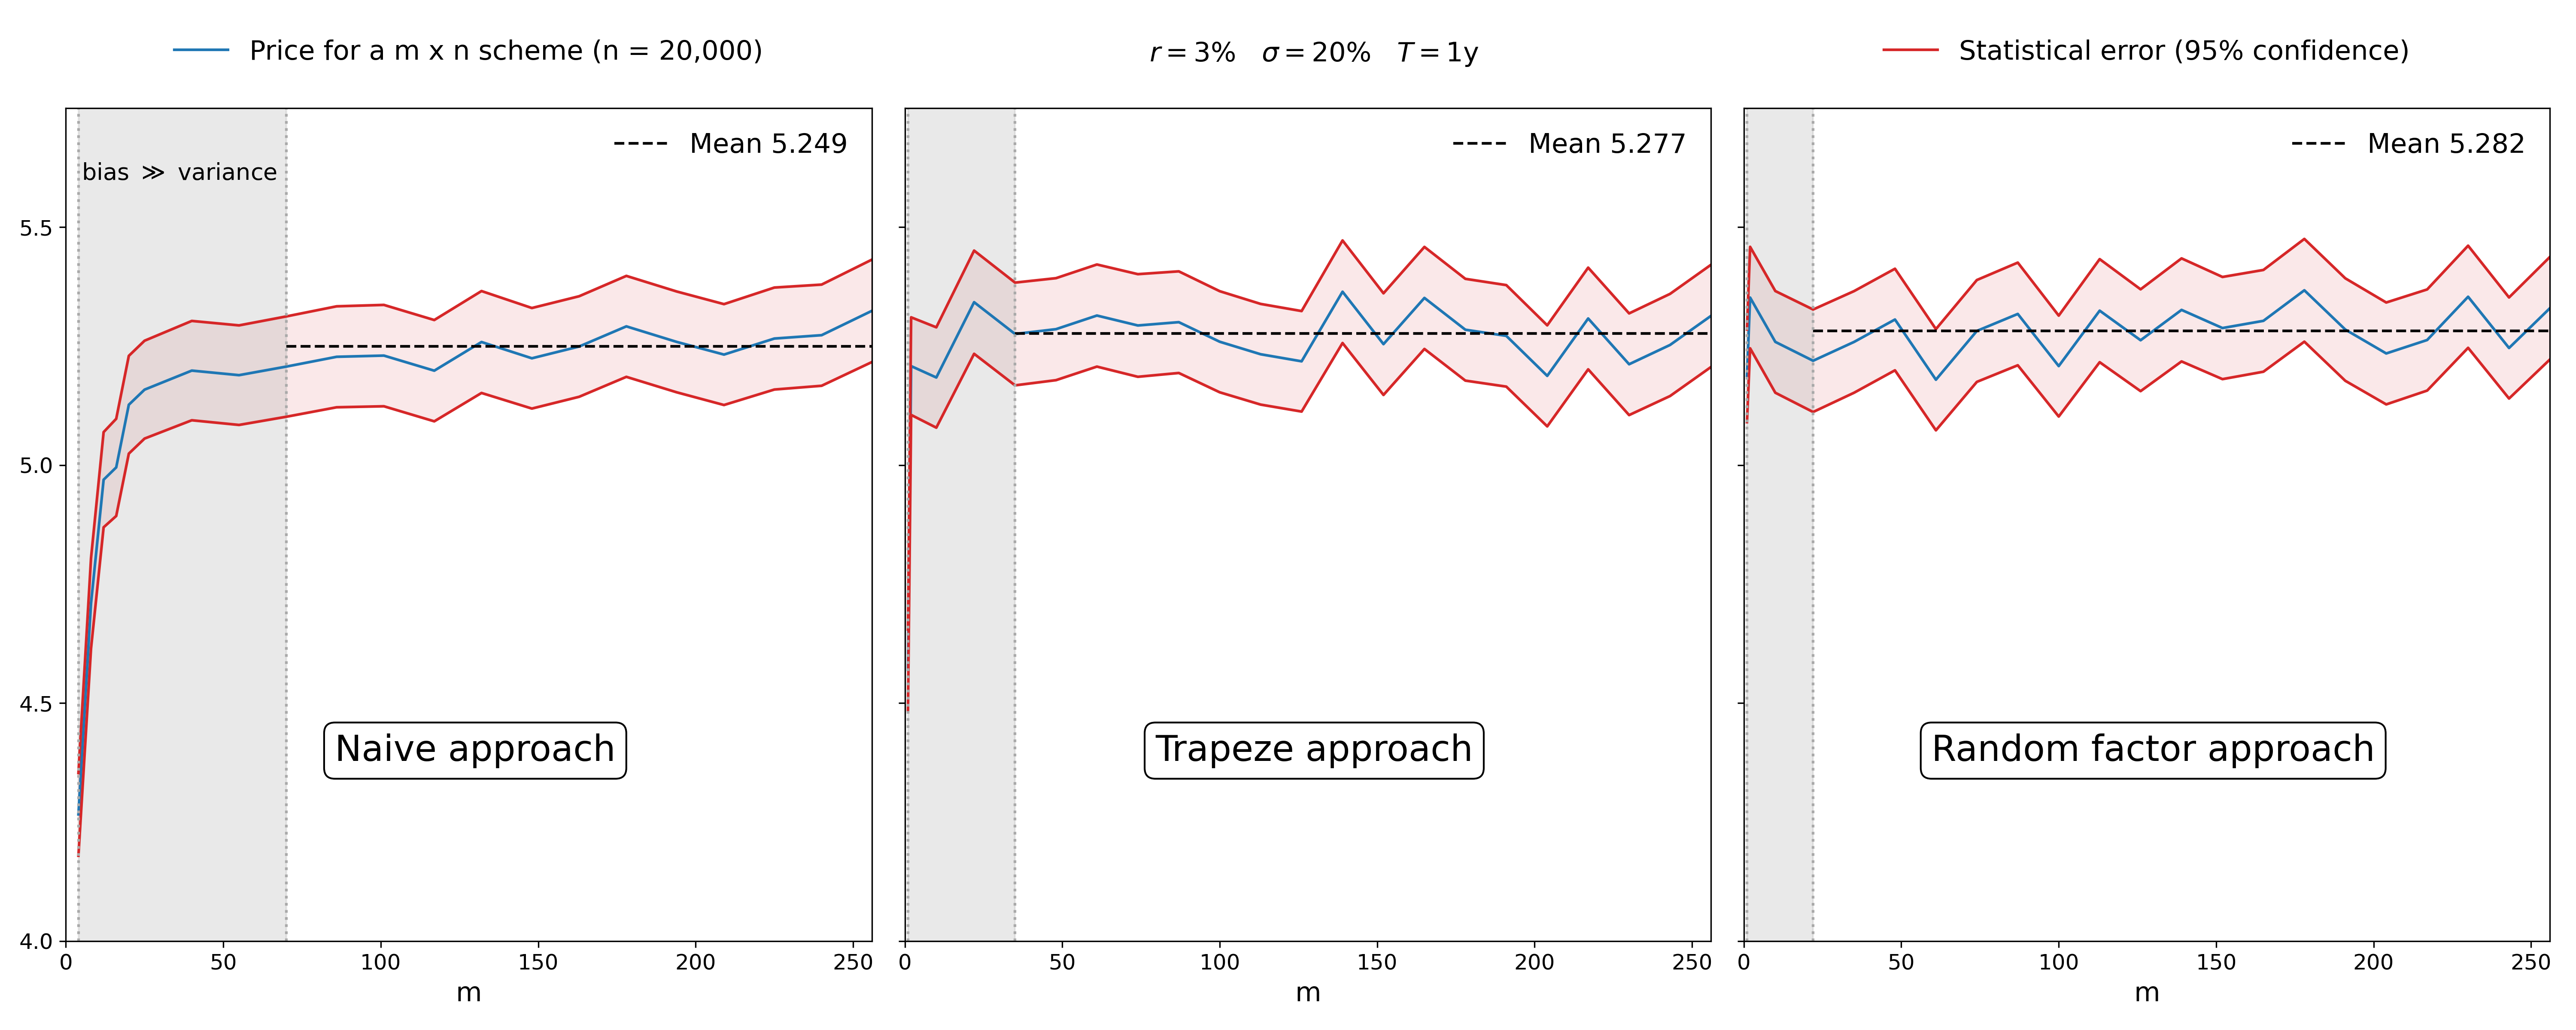
\includegraphics[width=1.04\textwidth]{charts/cvgce_wo_control.png}
  \caption{Convergence of schemes (1)-(3) for different values of $m$}
\end{figure}

\textbf{Description to be completed}.

\subsection{The use of a control variate}

In order to improve the convergence speed, Lambert et al. \cite{main} finally propose a variance reduction technique
for the three schemes above. It uses a control variate as introduced by Kemna et al. \cite{Vorst}.

\begin{equation}
	\theta = \sum_{i=1}^n \left( e^{-rT} \left[ A_T^i - K \right]_+ + \beta \left( Z^i - \mathbb E [Z] \right) \right)
	\tag{$\ast$}
\end{equation}

Observing that $e^x \approx 1 + x$ and $\ln(1 + x) \approx x$ when $| x |$ is small,
the idea relies on the approximation:
\[
	A_T = \frac{1}{T} \int_0^T S_u du \approx \exp \left\{ \frac{1}{T} \int_0^T \ln S_u du \right\}
	= S_0 \exp \left\{ \frac{1}{T} \int_0^T \ln \frac{S_u}{S_0} du \right\}
\]
The equality on the right-hand side justifies the validity of such approximation: if $r$ and $\sigma$ are small,
$S_u$ can be expected to remain near $S_0$ and $\ln \frac{S_u}{S_0} \ll 1$.
Therefore, we would like to use the following as a control variate in the case of a fixed-strike Asian call:
\[
	Z
	= e^{-rT} \left[ S_0 \exp \left\{ \left( r - \frac{\sigma^2}{2} \right) \frac{T}{2} +
		\frac{\sigma}{T} \int_0^T W_u du \right\}
		- K \right]_+
\]

Note that we can indeed compute the exact expression of $\mathbb E[Z]$. First, It\^o's lemma
gives $d(tW_t) = tdW_t + W_tdt$ and:

\[
	\frac{1}{T} \int_0^T W_u du = \frac{1}{T} \int_0^T (T-s) dW_s \sim \mathcal N \left(0, \frac{T}{3} \right)
	\quad \text{because} \quad \int_0^T (T-s)^2 ds = \frac{T^3}{3}
\]

If we note $a := \left( r - \frac{\sigma^2}{2} \right) \frac{T}{2}$, $b := \sigma \sqrt{\frac{T}{3}}$, $\rho :=\frac{K}{S_0}$,
$x^\ast := \frac{\ln \rho - a}{b}$ and $N$ the c.d.f of $\mathcal N (0, 1)$ then:
\begin{align*}
	\frac{\mathbb E[Z]}{e^{-rT} S_0}
	&= \int_{x^\ast}^{+ \infty} \left( e^{a + bx} - \rho \right) N'(x) dx \\
	&= e^{a + \frac{b^2}{2}} \int_{x^\ast - b}^{+ \infty} N'(u) du - \rho \int_{x^\ast}^{+ \infty} N'(x) dx
	\quad \text{with} \quad u = x - b \\
	&= e^{a + \frac{b^2}{2}} N(b - x^\ast) - \rho N(-x^\ast)
\end{align*}
	
On can check that the same computations yield Black-Scholes formula for the price of a European call.
Thus, we have the analytical expression. We finally need to provide a way to simulate the control variate $Z$
in each scenario. We define:

\begin{equation}
	\bar Z^{r, m} = e^{-rT} \left[ S_0 \exp \left\{ \left( r - \frac{\sigma^2}{2} \right) \frac{T}{2} +
		\frac{\sigma}{m} \sum_{i=0}^{m-1} \bar W_{t_k}^m \right\} - K \right]_+
	\tag{$i$}
\end{equation}

Plugging $\bar A_T^{r, m}$ from scheme $(1)$ and $\bar Z_T^{r, m}$ in $(\ast)$ yields a new scheme:
\begin{equation}
	e^{-rT} \left[ \bar A_T^{r, m} - K \right]_+ + \hat\beta_r \left( \bar Z_T^{r, m} - \mathbb E [Z] \right)
	\tag{4}
\end{equation}
where $\hat\beta_r$ is estimated with the empirical covariance of the variables.

\subsection{The combination of both improvements}

As we did with scheme $(1)$, we can plug the estimates of schemes $(2)$ and $(3)$ in $(\ast)$. That requires
to adapt the estimates of $Z$ too.
\begin{equation}
	\bar Z^{e, m} = e^{-rT} \left[ S_0 \exp \left\{ \left( r - \frac{\sigma^2}{2} \right) \frac{T}{2} +
		\frac{\sigma}{n} \sum_{i=0}^{n-1} \frac{\bar W_{t_{k+1}}^m + \bar W_{t_k}^m}{2} \right\} - K \right]_+
	\tag{$ii$}
\end{equation}
\begin{equation}
	\bar Z^{p, m} = e^{-rT} \left[ S_0 \exp \left\{ \left( r - \frac{\sigma^2}{2} \right) \frac{T}{2} +
		\frac{\sigma}{n} \sum_{i=0}^{n-1}
		\int_{t_k}^{t_{k+1}} \left( \bar W_u^m - \bar W_{t_k}^m \right) du
		\right\} - K \right]_+
	\tag{$iii$}
\end{equation}

It yields two new schemes.

\section{PDE approaches}

\section*{Conclusion}


\bibliography{bibliography}{}
\bibliographystyle{plain}

\end{document}